\begin{flushright} {\tiny {\color{gray} python\_codes/fieldstone\_121/text.tex}} \end{flushright}

%\lstinputlisting[language=bash,basicstyle=\small]{python_codes/fieldstone_01/keywords}

\begin{center}

\fbox{\textbf{\huge \color{teal} P}}
Code at \url{https://github.com/cedrict/fieldstone/tree/master/python_codes/fieldstone_121}
\end{center}

\par\noindent\rule{\textwidth}{0.4pt}

%%%%%%%%%%%%%%%%%%%%%%%%%%%%%%%%%%%%%%%%%%%%%%%%%%%%%%%%%%%%%%%%%%%%%%%%%%%%%%%%%%%%%%%%%%%%%%%%

The domain is a 2D Cartesian box of size $L_x \times L_y$ with 
$L_x=200~\si{\km}$ and $L_y=100~\si{\km}$.
The isothermal incompressible Stokes equations are solved on a mesh 
of $nelx\times nely$ $Q_2\times Q_1$ elements (same as \aspect).
 

It contains a single fluid characterised by the dislocation creep 
effective viscosity of \textcite{gatt20} (2020) and \textcite{gath21} (2021):
\[
\eta_{disl}(\dot{\varepsilon}_e,T)  = \frac{A_0}{2\dot{\varepsilon}_e}\left[ 
1 + \tanh\left( A_1 ( \log_{10}   \dot{\varepsilon}_e - A_2 )  \right)
\right]
\]
with 
\begin{align}
A_0(T) &= a_0 + b_0 T \nn\\ 
A_1(T) &= a_1 + b_1 T \nn\\ 
A_2(T) &= a_2 + b_2 T +c_2T^2 \nn
\end{align}
and
\begin{align}
a_0 &= 4.4\cdot 10^8 \nn\\
b_0 &= -5.26\cdot 10^4 \nn\\
a_1 &= 2.11\cdot 10^{-2} \nn\\
b_1 &= 1.74\cdot 10^{-4} \nn\\
a_2 &= -41.8 \nn\\
b_2 &= 4.21\cdot 10^{-2} \nn\\
c_2 &= -1.14\cdot 10^{-5} \nn
\end{align}

The setup is similar to the one in \textcite{gupm14} (2014) although the formulation here is purely 
Eulerian and will rely on periodic boundary conditions when large shear values are used.
Boundary conditions are $\vec{\upnu}=(+u_0,0)$ on the top, $\vec{\upnu}=(-u_0,0)$ on the 
bottom, and $v=0$ on the left and right boundaries. We thereby obtain a flow 
that is parallel to the $x$-axis. $u_0$ is set to $1~\si{\cm\per\year}$.

The rheology is nonlinear so Picard nonlinear iterations are implemented. These stop
when the difference between two consecutively obtained velocity fields falls below
a given tolerance $tol=10^{-3}$. 

The temperature field is set to a constant value $T_0$ throughout the domain.

If no thermal or mechanical inhomogeneity is implemented, this setup results in 
a velocity field $\vec{\upnu}=(u,v)$ that is such that $v(x,y)=0$, and 
$u(x,y)=2u_0 (y-L_y/2)/L_y$, with $\dot{\varepsilon}_{xx}=\dot{\varepsilon}_{yy}=0$ 
and $\dot{\varepsilon}_{xy}=u_0/L_y$. 

\begin{center}
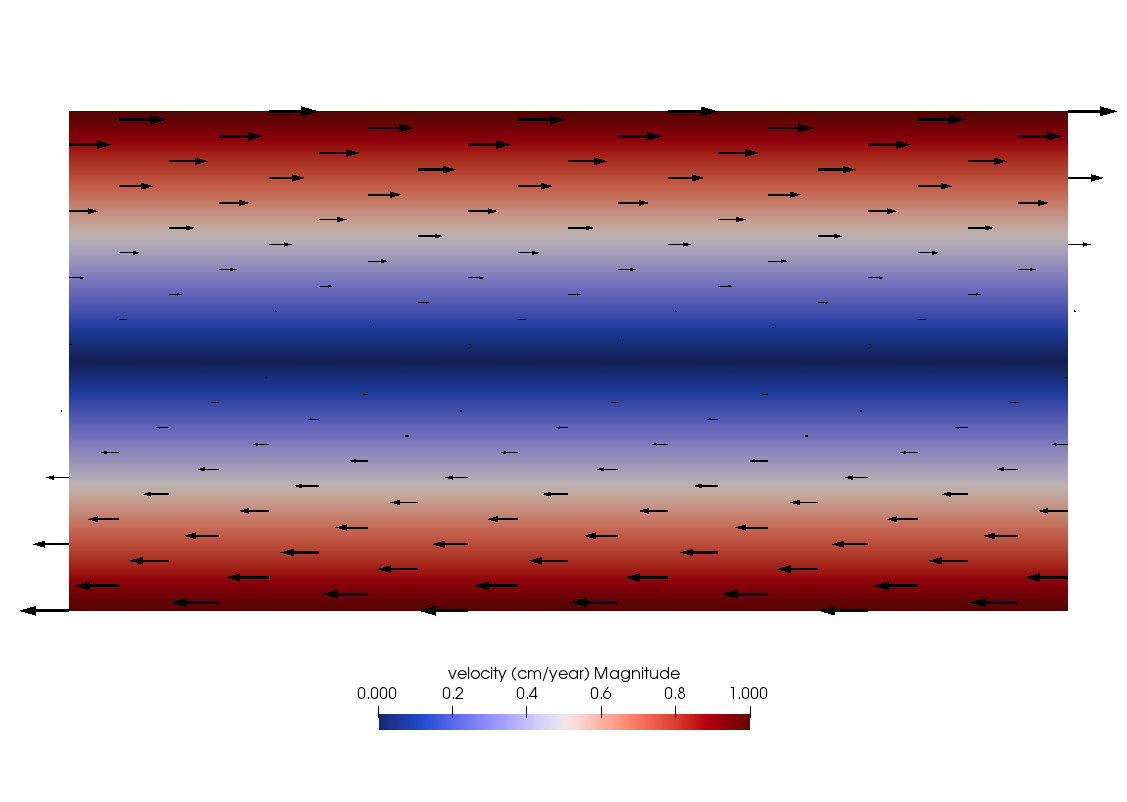
\includegraphics[width=7cm]{python_codes/fieldstone_121/results/vel}
\end{center}

We therefore need a form of weak seed/zone to localise the deformation and 
initiate the strain weakening process.

I will soon implement a passive set of particles on which strain can be accumulated so as 
to allow for strain weakening. What form should the strain weakening take?

PIC, markers, averaging 



\newpage
%%%%%%%%%%%%%%%%%%%%%%%%%%%%%%%%%%%%%%%%%%%%%%%%%%%%%%%%%%%%%%%%%%%%%%%%%%%%%
\section*{Project rheology: Strain localisation a la \textcite{gupr14}}

The deformation mechanism equations are from \textcite{gupr14} (2014):
\[
\dot\varepsilon = \dot\varepsilon_{dsl} + \dot\varepsilon_{dif} + \dot\varepsilon_{gbs} + \dot\varepsilon_{exp} 
\]
with
\begin{eqnarray}
\dot\varepsilon_{dsl}&=&A_{dsl}\exp\left(-\frac{Q_{dsl}}{RT} \right) \tau^{n_{dsl}}  \\
\dot\varepsilon_{dif}&=&A_{dif}\exp\left(-\frac{Q_{dif}}{RT} \right) \tau^{n_{dif}} d^{m_{dif}} \\
\dot\varepsilon_{gbs}&=&A_{gbs}\exp\left(-\frac{Q_{gbs}}{RT} \right) \tau^{n_{gbs}} d^{m_{gbs}} \\
\dot\varepsilon_{exp}&=&A_{exp}\exp\left[-\frac{Q_{exp}}{RT} \left(1 -\frac{\tau}{\tau_p}\right)^{n_{exp}} \right]   
\end{eqnarray}
where $d$ is the grain size, $m$ is the grain size exponent, $\tau_p$ is the Peierls stress defined
for low-temperature plasticity.

We will come back to how the strain rate partitioning is done later. 
Assuming the strain rate known (as well as the temperature) these relationships can 
be reversed so as to give the stress as a function of strain rate and temperature:
\begin{eqnarray}
\tau &=& A_{dsl}^{-1/n_{dsl}} \dot\varepsilon_{dsl}^{1/n_{dsl}}  \exp \left(\frac{Q_{dsl}}{n_{dsl} RT} \right)  \\
\tau &=& A_{dif}^{-1}         \dot\varepsilon_{dif}              \exp \left(\frac{Q_{dsl}}{        RT} \right) d^{-mdif/ndif} \\
\tau &=& A_{gbs}^{-1}         \dot\varepsilon_{gbs}              \exp \left(\frac{Q_{gbs}}{        RT} \right) d^{-mgbs/ngbs} \\
\tau &=& A_{exp}
%\dot\varepsilon_{exp}&=&A_{exp}\exp\left[-\frac{Q_{exp}}{RT} \left(1 -\frac{\tau}{\tau_p}\right)^{n_{exp}} \right]   
\end{eqnarray}


\begin{center}
\begin{tabular}{lllllll}
\hline
& $A$ & $Q$ & $n$ & $m$ & $\tau_p$ & ref. \\
\hline\hline
 & $\si{\mega\pascal^{-n}\per\second}$ & $\si{\kilo\joule\per\mole}$ &&& \si{\mega\pascal}?\\
\textbf{Mantle} (olivine)  &  \\ 
Dislocation       & $1.1\cdot10^5$    &530& 3.5 & -  &-   &\cite{hiko03}\\
Diffusion         & $3.98\cdot 10^7$  &370& 1   & 3  &-   &\\
Dry GBS           & $6.5\cdot10^3$    &400& 3.5 & 2  &-   &\\
Dry GBS           & $6.31\cdot10^4$   &445& 2.9 & 0.7&-   &\cite{hazk11}\\
Exponential       & $5.7\cdot10^{11}$ &535& 2   & -  &8500&\cite{goet78}\\
\hline
\textbf{Crust} (quartz) &\\
Dislocation (weak)   &  $3.2\cdot10^{-4}$    & 154 & 2.3&- & - & \cite{kikr87}\\
Dislocation (strong) &  $6.31\cdot 10^{-12}$ & 135 & 4&- & - & \cite{hitd01}\\
\hline
\end{tabular}
\end{center}

\begin{center}
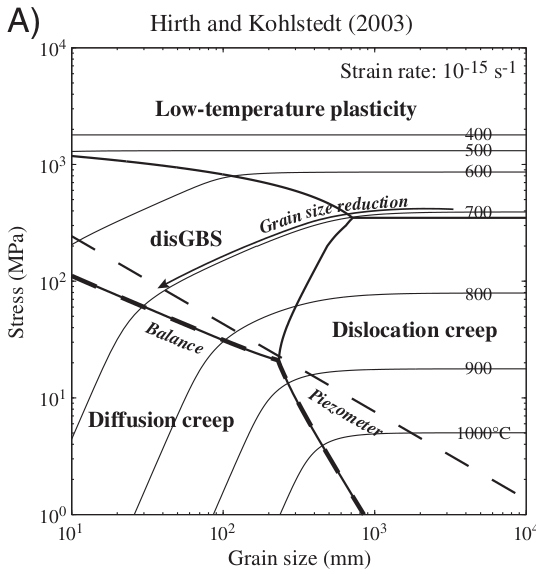
\includegraphics[width=7cm]{python_codes/fieldstone_121/images/gupr14a}
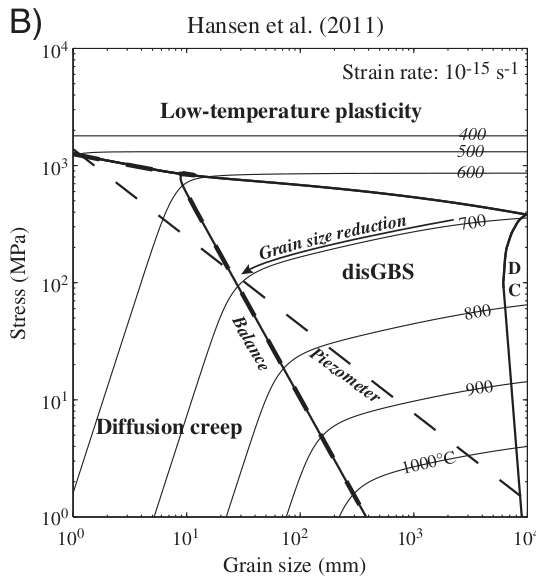
\includegraphics[width=7cm]{python_codes/fieldstone_121/images/gupr14b}\\
{\captionfont Taken from \textcite{gupr14} (2014). Olivine deformation maps 
(shear stress vs. mean grain size) at a constant strain rate ($10^{-15}~\si{\per\second}$) 
showing the four deformation mechanisms that compete to control the mantle rheology: 
low-temperature plasticity (exponential creep), dislocation creep, disGBS
and diffusion creep. Iso-temperature curves are provided to show stress/grain sizes for
temperatures ranging from 1000 to 400~\si{\celsius}. 
A) deformation map including the disGBS
flow law from \textcite{hiko03} (2003); 
B) deformation map including the disGBS flow law from \textcite{hazk11} (2011). 
Hypotheses for the recrystallized grain size are either
equilibrium (at the boundary between grain size sensitive and grain size insensitive
creeps, thick dashed line; de Bresser et al., 1998) or experimentally constrained paleo-
piezometer (thin dashed line; Van der Wal et al., 1993). Values of the ductile flow laws
are given in the Table above}
\end{center}


\newpage
%%%%%%%%%%%%%%%%%%%%%%%%%%%%%%%%%%%%%%%%%%%%%%%%%%%%%%%%%%%%%%%%%%%%%%%%%%%%%
\section*{Project inclusion}

The domain is $1~\si{\cm}$ thick. It contains two materials:
\begin{itemize}
\item material 1: ab $A=$, $n=$, $Q=$ (the matrix)
\item material 2: cpx $A=$, $n=$, $Q=$ (the inclusion)
\end{itemize}
The effective viscosity is computed assuming a dislocation creep mechanism
in which pressure dependence has been removed:
\[
\eta_{eff} = A^{-1/n} \dot{\varepsilon}^{-1+1/n} \exp\left( \frac{Q}{nRT}\right)
\]
The temperature is assumed to be constant in the domain, i.e. $T=T_{background}$.
Boundary conditions are $\vec{\upnu}=(+u_0,0)$ on the top, $\vec{\upnu}=(-u_0,0)$ on the 
bottom, and $v=0$ on the left and right boundaries. We thereby obtain a flow 
that is parallel to the $x$-axis. $u_0$ is set so that the strain rate is $10^{-15}~\si{\per\second}$.

A single inclusion of radius $R_i$ is placed in the middle of the domain.

The particle in cell technique is used here in combination with 
periodic boundary conditions in the horizontal direction.
Viscosity is computed on each particle and then these particle-based 
viscosities are projected onto the quadrature points (note: many options to 
explore here - elemental averaging is used for now). 
Because the viscosity depends on the strain rate, this makes the equations 
to be solved nonlinear. We deal with this by resorting to Picard iterations. 
Nonlinear iterations stop when a given tolerance ({\tt tol}) is reached or when the 
allowed maximum number of iterations is reached ({\tt niter}).

Time stepping is implemented and the value of the timestep $\delta t$ is obtained 
by means of a CFL condition, controlled by the CFL coefficient {\tt CFL\_nb} which 
should remain somewhere between 0 and 0.5. For simplicity a first order Euler scheme is implemented 
for the advection of these particles . 

\vspace{1cm}

FUTUR stuff:
Following \textcite{begu18} (2018), we 
express pore fluid pressure variations using Darcy’s law and the fluid mass 
conservation (Gratier et al., 2003) leading to 
\[
\phi_m C \frac{\partial P_f}{\partial t}
+\frac{\partial \phi_m}{\partial t}
= 
\frac{\partial}{\partial x} K \frac{\partial P_f}{\partial x} + F
\]
where $\phi_m$ is the mean porosity, $C$ is the mean matrix-fluid compressibility, 
$t$ is time, $x$ is the distance across the
shear zone, $K$ is the permeability, and $F$ is the fluid pumping parameter. 
We relate porosity and permeability following \textcite{skre16} (2016):
\[
K = K_0 \left( \frac{\phi}{\phi_0} \right)^{\alpha_k}
\]
where $K_0$ is the permeability at a reference porosity $\phi_0$ 
and $\alpha_k$ is the permeability exponent
(set here to 3, see \textcite{skre16} 2016)

Observations on midcrustal granitic shear zones show that porosity concentrates
along grain boundaries and decreases with the distance to the core of the shear zone (Fusseis et al., 2009).
Therefore, we assume that porosity is inversely proportional to grain size (see supporting information S2).

Finally, we model the enhancement of fluid pumping by ductile deformation as
\[
\dot{F} = \phi_f F \dot{\varepsilon}
\]
where $F$ is the fluid pumping and $\phi_F$ is the kinematic of the fluid pumping. 
The strain rate-dependent fluid pumping assumption is required to describe both strong 
fluid circulation in the core of the shear zone and nearly no fluid circulation at 
the rim. We set the kinematic of fluid pumping $\phi_F$ to $7\cdot10^4$ in order to have a 
characteristic time of fluid pumping of 5,000 days (~14 years). 
Note that a lower fluid pumping rate inhibits strain
localization described below while a larger fluid pumping rate implies numerical instabilities.


